\section{Results and Discussion}

From these kappa values we find that most classifiers' performances are not far away from random decisions ($\kappa$ <0.2 \cite{cohenskappa}). But there are still some features can help the classifier stop making random decisions. We run \emph{Student-t test} on the kappa values for each feature of each network to test the randomness of Kappa results. The t-test shows that only kappa result from Nonlinear Regression Analysis features ($p = 0.0409 < 0.05$, $\kappa$ values with $\mu = 0.0628, median = 0.0573,\sigma = 0.1387$) is significantly not random. If we look inside of each features of 216-channel Nonlinear Regression Analysis functional connectivity maps, we found that  216-channel Nonlinear Regression Analysis weighted feature of \emph{global efficiency} can give the best Kappa result with significance ($p = 0.0043$) of $0.1112 \pm 0.1673$.

\begin{figure}[!t]
    \centering
    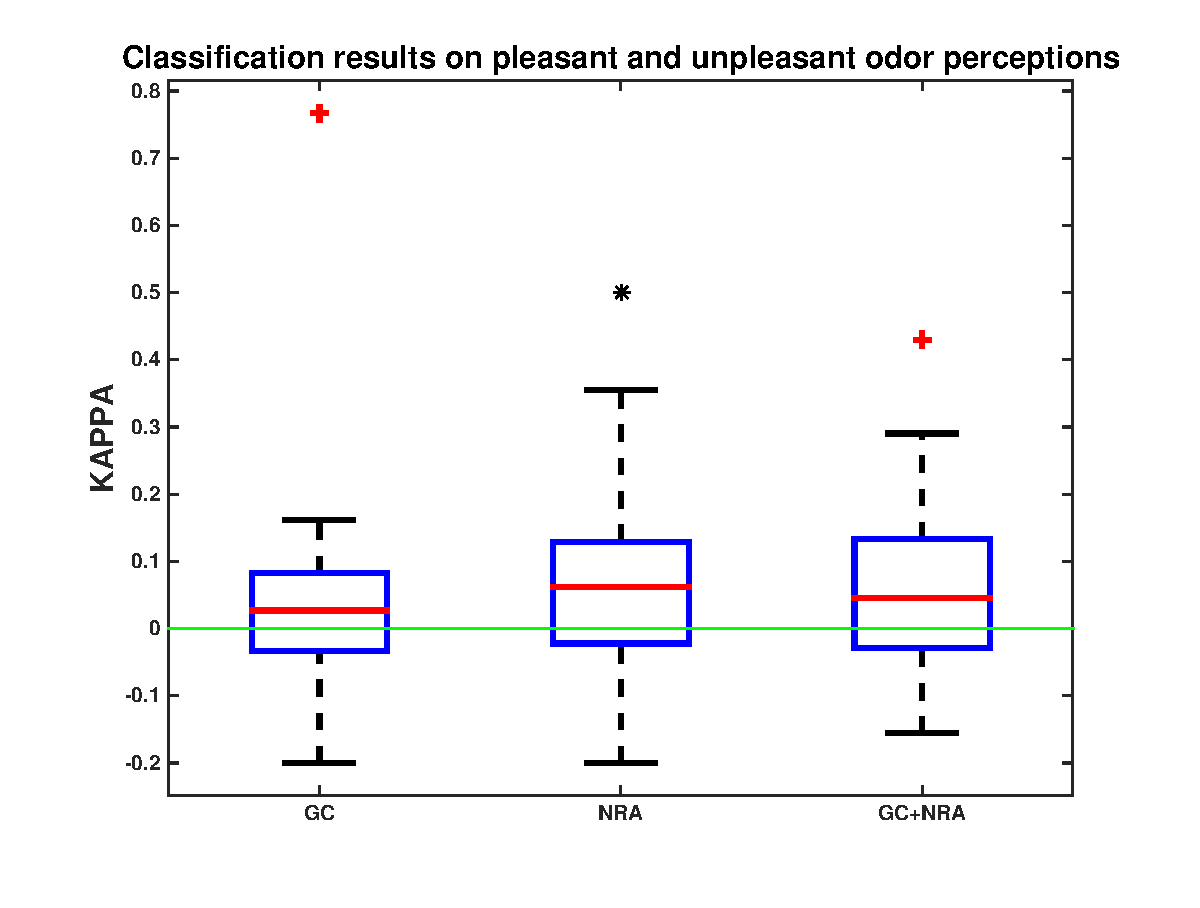
\includegraphics[width=0.45\textwidth]{./images/kappa.eps}
    \caption{Cohen's Kappa resluts boxplots. GC presnets the Cohen's Kappa resluts for Granger Causality method. NRA represents the Cohen's Kappa results for Nonlinear Regression Analysis method. GC+NRA represents the classification results using both Granger Causality and Nonlinear Regression Analysis methods.}
    \label{fig:kaapa}
\end{figure}

Although the significant kappa results have the $p-values$ less than 0.05, some of the $p-value$ are still very close to 0.05, indicating that the results are not that good anyway.The low classification accuracy may due to many reasons: the size of functional connectivity map may play a crucial rule in classification -- with 19-channel functional connectivity maps, there might be too less detail for connections while 216-channel functional connectivity maps may provide too much redundant information in classification. New features of functional connectivity maps should also be proposed. Since we only used network-based features in this paper, other features as power spectral density or time-frequency analysis may also be used for classification. Another improvement for getting better classification results could be done in the experiment design. Based on the experiment protocol and preprocessing of raw EEG signal, 6 seconds of each trial of EEG signal are kept fro investigating the pleasantness from odours. This time duration could be cut shorter (because 6 seconds might be to much for decision making) or extended longer (or because 6 seconds might be not enough to make the decision).